%%%%%%%%%%%%%%%%%%%%%%%%%%%%%%%%%%%%%%%%%%%%%%%%%%%%%%%%%%%%%%%
\section{Production and Assembly}
\label{sec:fdsp-pd-prod-assy}
\metainfo{(Length: TDR=40 pages, TP=8 pages)}

%%%%%%%%%%%%%%%%%%%%%%%%%%%%%%%%%%
\subsection{Photon Collectors Production}
\label{sec:fdsp-pd-prod-pc}
\metainfo{\color{blue} Content: Cavanna/Whittington/Machado}
	
\subsubsection{Dip-Coated Light Guides (2 pages)}
\label{ssec:fdsp-pd-pc-prod-bar1}

\subsubsection{Double-Shift Light Guides (2 pages)}
\label{ssec:fdsp-pd-pc-prod-bar2}

The production and assembly of the double-shift light guide modules is divided 
into separate threads for the wavelength-shifting plates and the EJ-280 light guides. 
Many of the production, quality assurance, and assembly procedures developed for the
 double-shift light guide design deployed at ProtoDUNE-SP will remain the same for 
the DUNE single-phase far detector.

\paragraph*{Manufacture of the WLS Plates}

Spray-coating of TPB on acrylic plates (see Fig.~\ref{fig:DoubleShiftLG-SprayedPlates}).

\begin{dunefigure}[TPB-coated acrylic plates after spraying at Indiana University during fabrication of parts for ProtoDUNE-SP.]{fig:DoubleShiftLG-SprayedPlates}
 {TPB-coated acrylic plates after spraying at Indiana University during fabrication of parts for ProtoDUNE-SP.}
  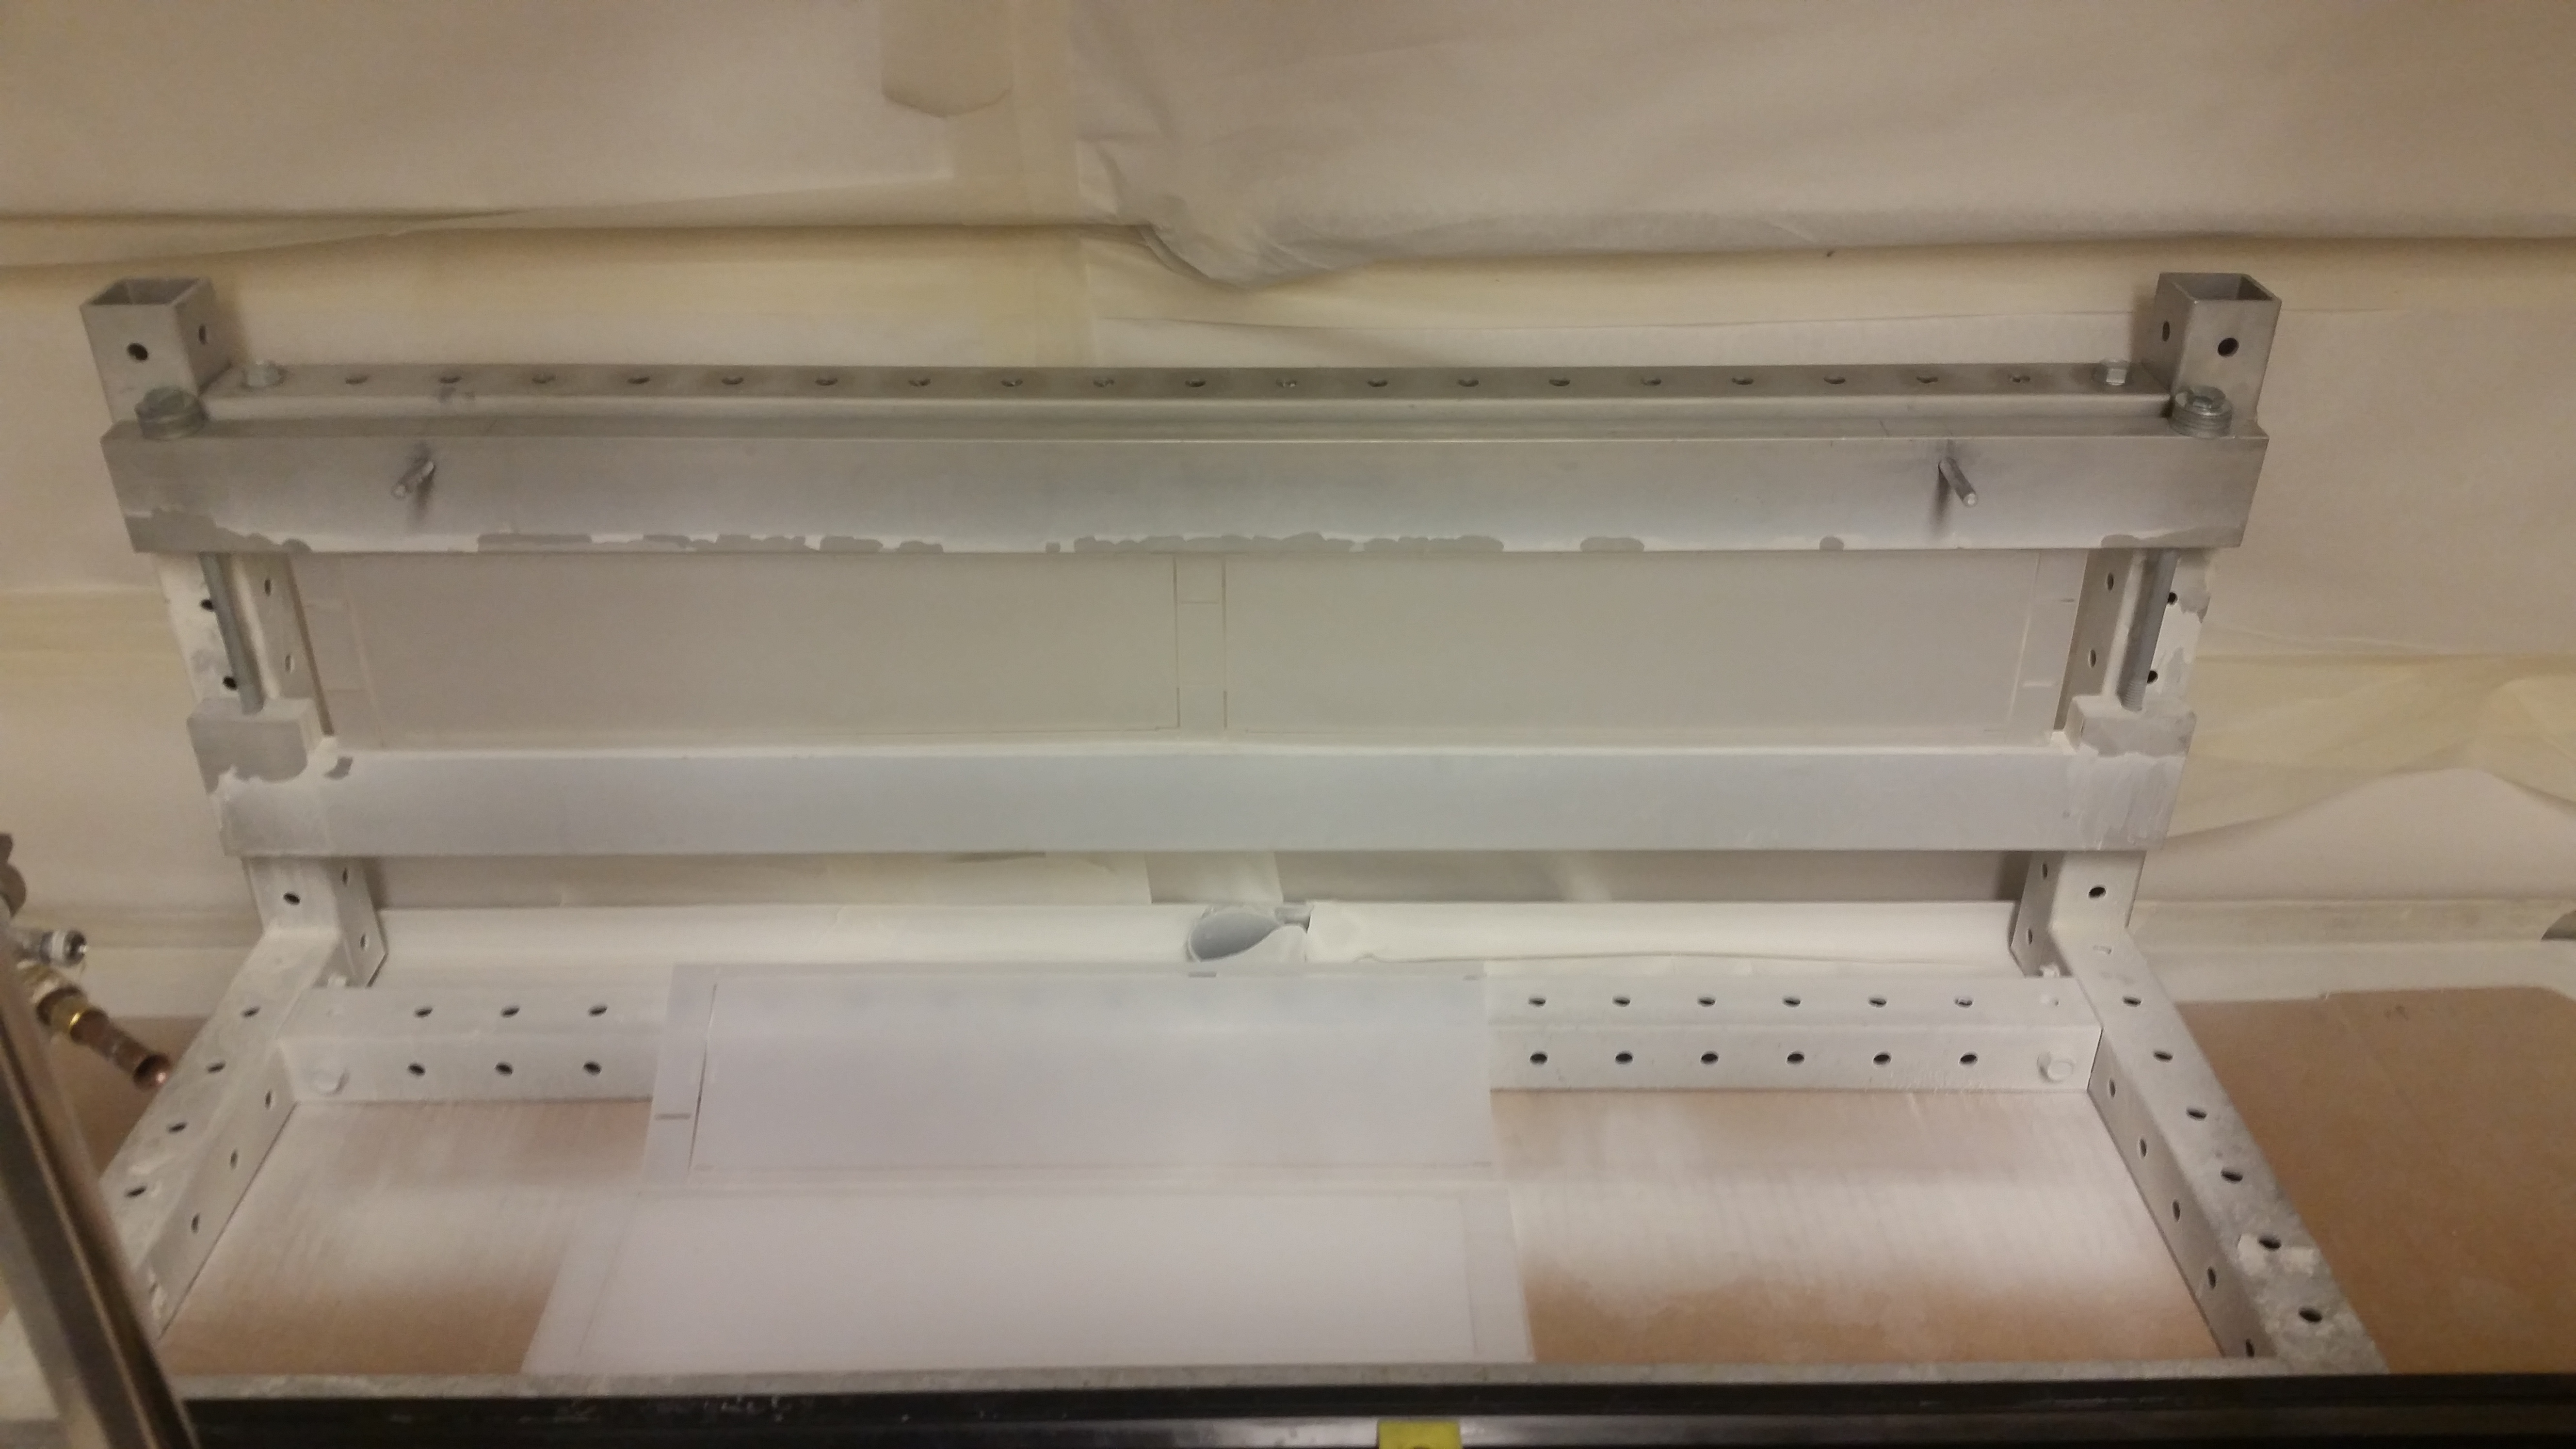
\includegraphics[width=0.7\columnwidth]{pds-DoubleShiftLG-SprayedPlates.jpg}
\end{dunefigure}

\paragraph*{QA of the WLS Plates}

VUV conversion performance measured for neighboring samples from the 
acrylic plate template using a vacuum-ultraviolet monochromator.

\paragraph*{Receipt and QA of the Light Guides}

EJ-280 light guides fabricated by Eljen Technologies. Received and scanned in a 
long dark-box using a blue LED~(Fig.~\ref{fig:DoubleShiftLG-EJ280}).
 Measure conversion and transmission to the light guide ends to test attenuation. 
Direct transmission through the light guide to confirm uniformity. 
Attenuation length in liquid argon shorter than in air, but long attenuation in 
air has been shown to correspond to long attenuation in liquid argon.

\begin{dunefigure}[EJ-280 light guide within darkbox for attenuation scan QA at Indiana University (prepared for ProtoDUNE-SP).]{fig:DoubleShiftLG-EJ280}
{EJ-280 light guide within darkbox for attenuation scan QA at Indiana University (prepared for ProtoDUNE-SP).}
  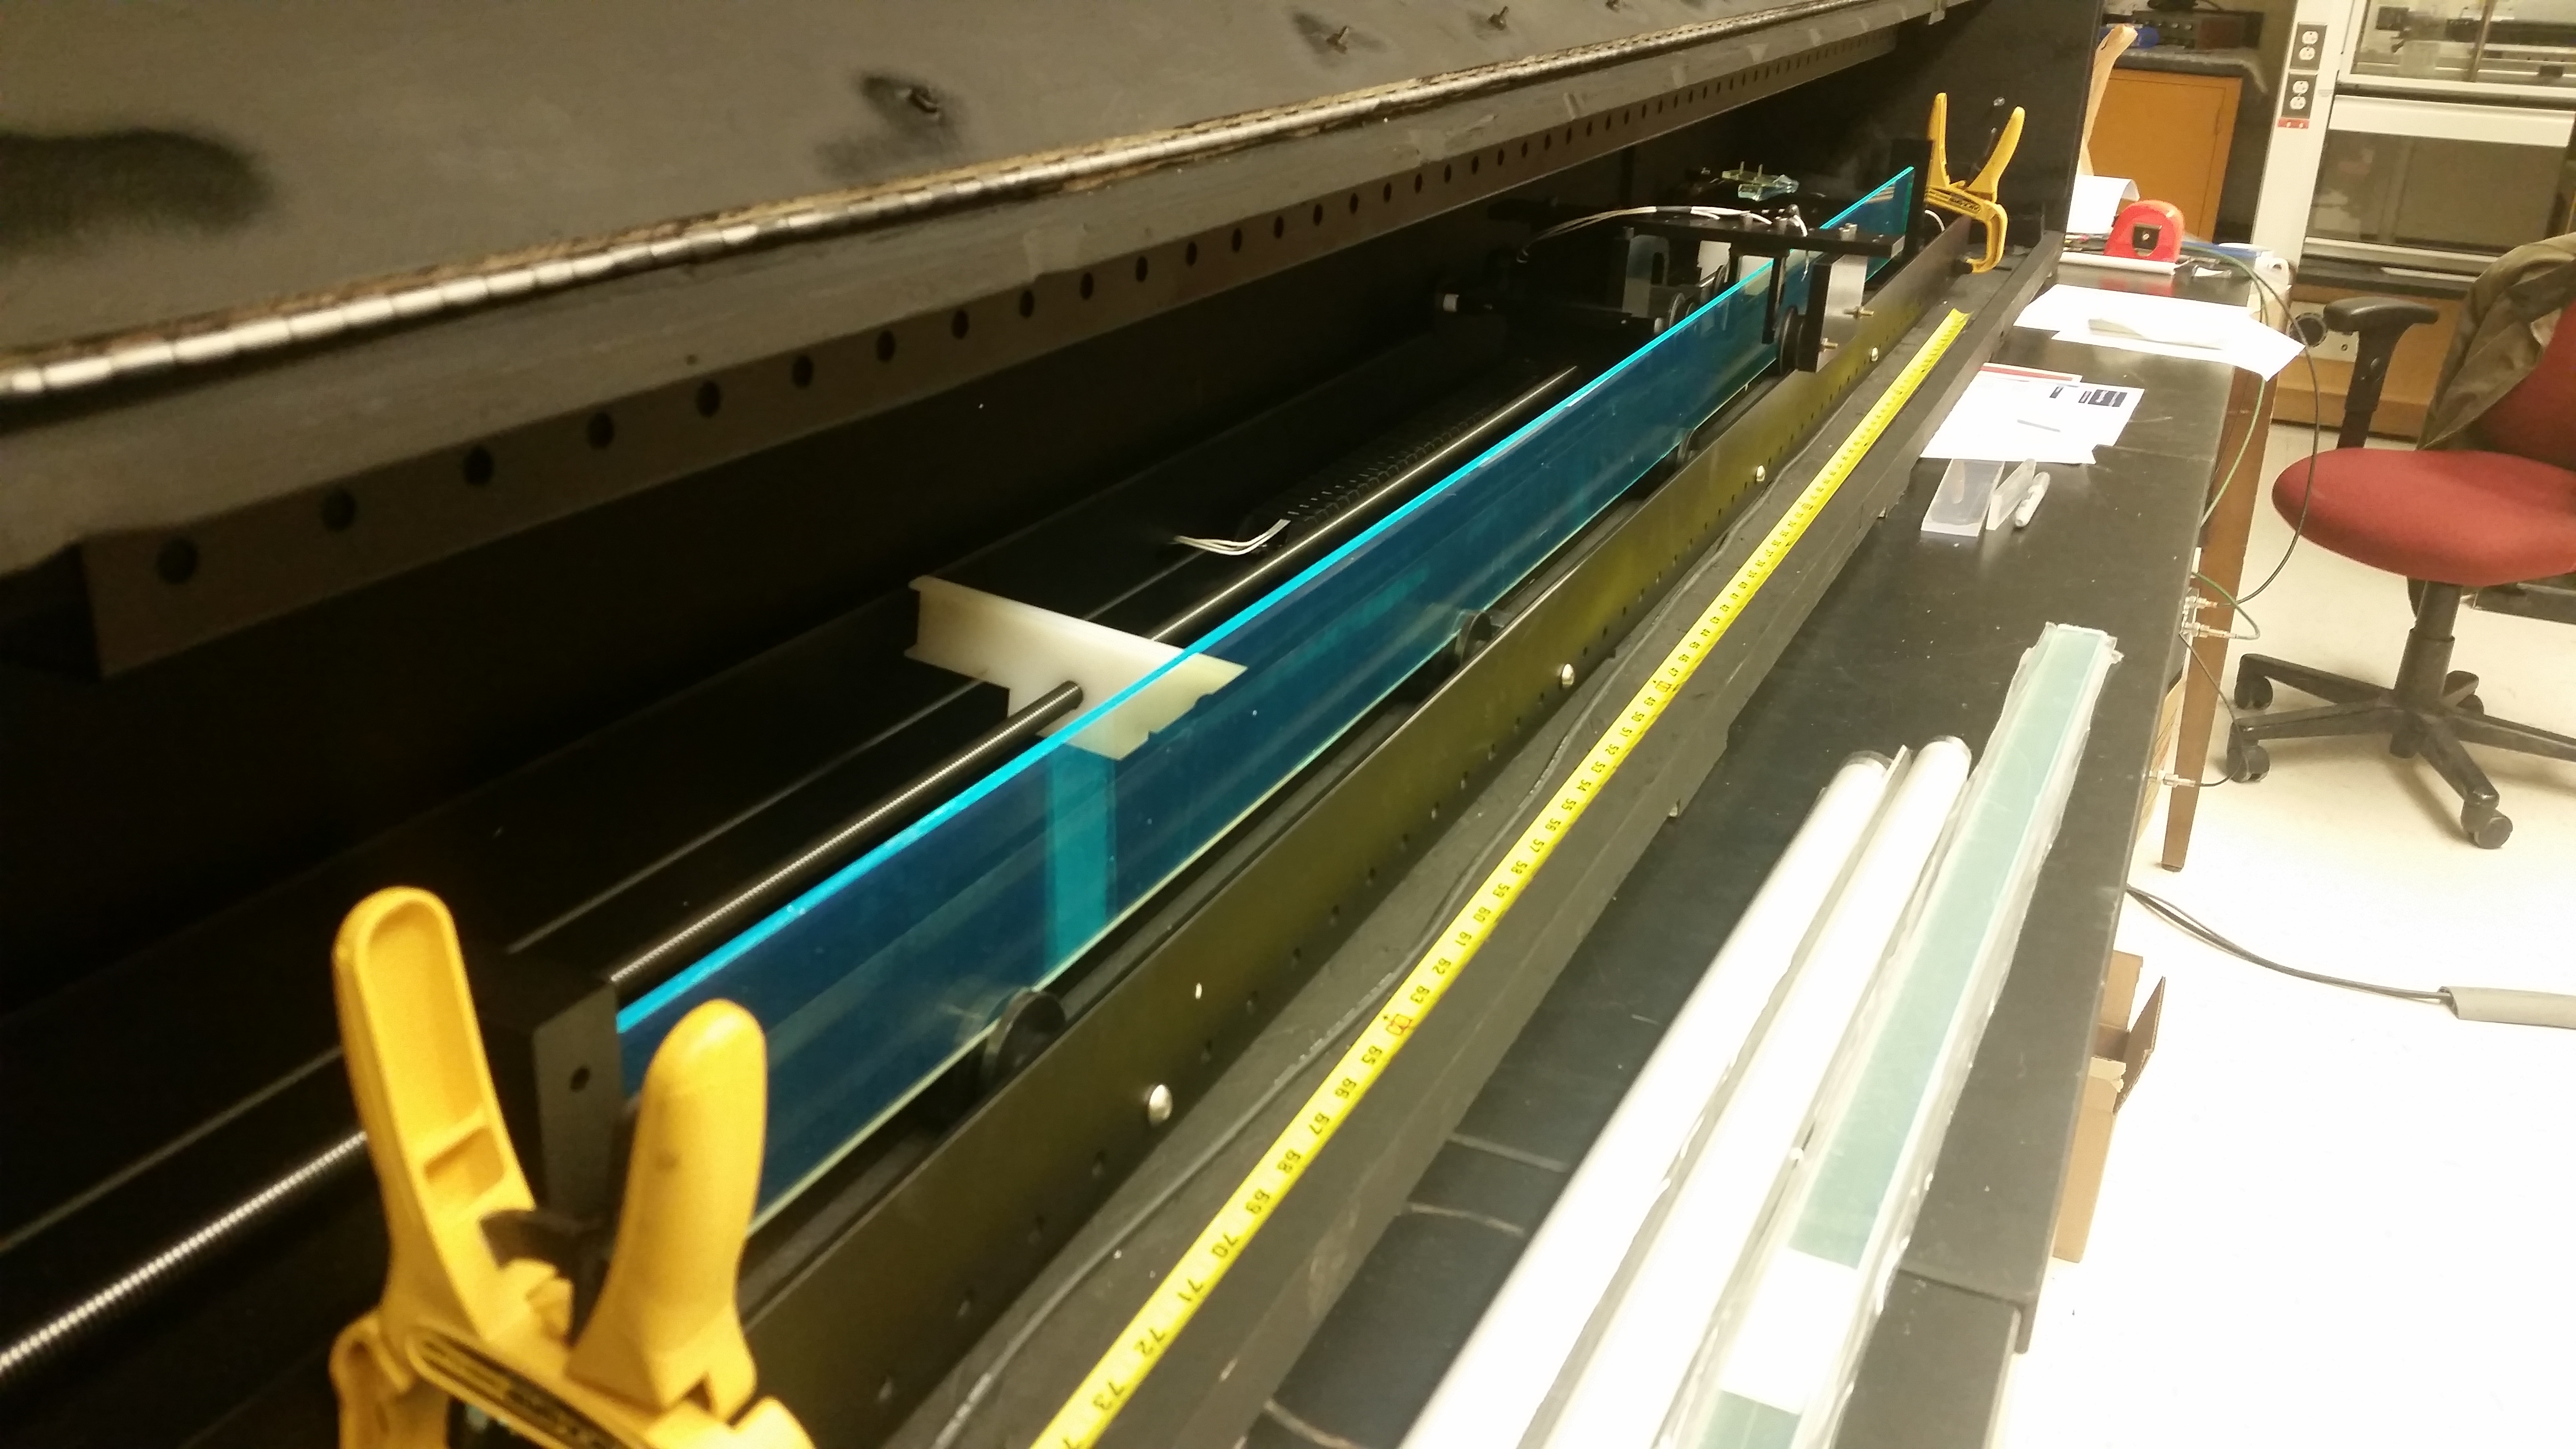
\includegraphics[width=0.6\columnwidth]{pds-DoubleShiftLG-EJ280.jpg}
\end{dunefigure}

\paragraph*{Assembly of the Double-shift Light Guide Module}

Parts are shipped to the assembly point where the EJ-280 light guide is mounted 
into the module frame and the WLS plates are attached.

\begin{dunefigure}[Mounting of the WLS plates to the EJ-280 bar.]{fig:DoubleShiftLG-PlateMounting}
{Mounting of the WLS plates to the EJ-280 bar.}
  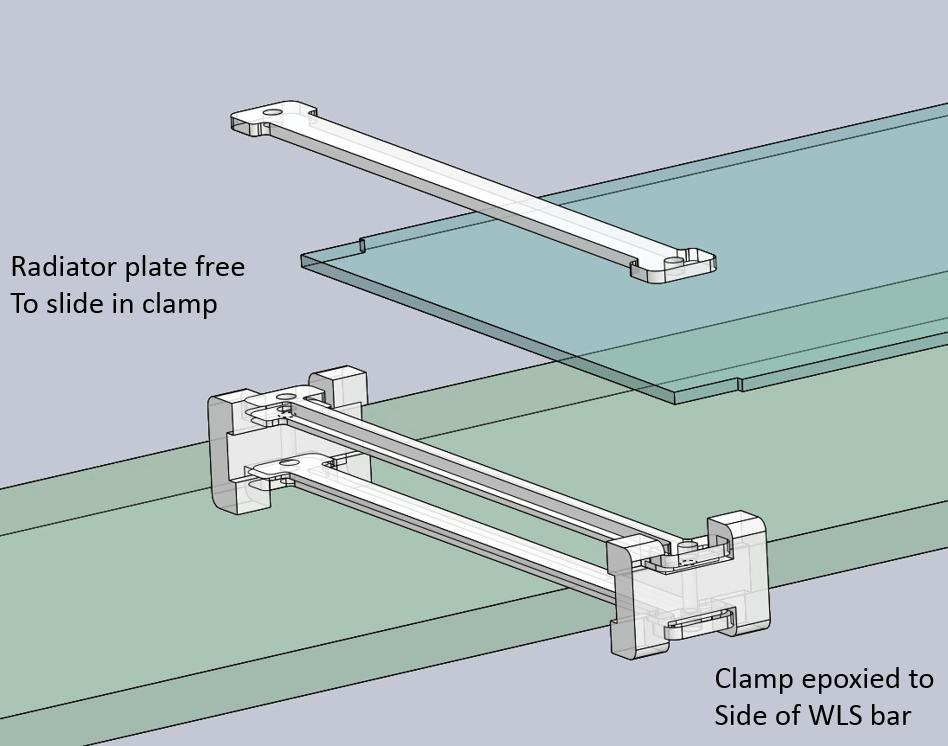
\includegraphics[width=0.5\columnwidth]{pds-DoubleShiftLG-PlateMounting.jpg}
\end{dunefigure}


\subsubsection{ARAPUCA (2 pages)}
\label{ssec:fdsp-pd-pc-prod-arapuca}



%%%%%%%%%%%%%%%%%%%%%%%%%%%%%%%%%%
%\subsection{PD Mounting in APA Frames}
\subsection{APA Frame Mounting Structure and Module Fixing}	
\label{sec:fdsp-pd-assy-frames}
\metainfo{\color{blue} Content:   (2 pages) - Warner}

Photon detector (PD) modules are inserted into the APA frames through ten slots 
(five on each side of the APA frame) and are supported in place inside the frame in 
stainless steel guide channels.  The slot dimensions for the ProtoDUNE APA frames 
were 108.0mm X 19.2mm wide (See fig. 1).  The guide channels are pre-positioned into 
the APA frame prior to applying the wire shielding mesh to the APA frames, and are
not accessible following wire wrapping.

\fixme{Insert Dave's PD Mounting rails in APA frame mpicture}

Following insertion, the PD modules are fixed in place in the APA frame using
 two stainless steel captive screws, as shown in figure 2.

\fixme{Insert Dave's PD Mounting screws mpicture}

\subsubsection{Cryogenic thermal contraction}

Bar-style PD modules are structurally composed of primarily polycarbonate and 
acrylic, which have significantly different shrinkage factors compared to the 
stainless steel APA and PD support frames (see table 1).

\fixme{format table better?}

\begin{table}[h!]
\label{tbl:fdsfpdshrink}
\begin{center}
\caption{Shrinkage of Photon Detector Materials}
\begin{tabular}{|c|c|}
\hline
\textbf{Material Shrinkage Factor (m/m)} & \textbf{$206^{\circ}C$ Drop}\\
\hline
Stainless Steel (304) & $2.7\times10^{-3}$\\
FR-4 G-10 (In-plane) & $2.1\times10^{-3}$\\
Polystyrene (Average) & $1.5\times10^{-2}$\\
Acrylic and Polycarbonate (Average) & $1.4\times10^{-2}$\\
\hline
\end{tabular}
\end{center}
\end{table}

These differences in thermal expansion (or contraction in this case) were 
important to keep in mind during design of the PD module supports.  
Mitigation for these varying contractions are detailed in table 2:

\fixme{ Needs better table formatting? }

\begin{table}[h!]
\label{tbl:fdsfpdshrinkeffects}
\begin{center}
\caption{Relative Shrinkage of PD components and APA frame, and mitigations}
\begin{tabular}{|p{0.25\textwidth}|p{0.25\textwidth}|p{0.4\textwidth}}
\hline
\textbf{Interface} & \textbf{Relative shrinkage} & \textbf{Mitigation} \\
\hline
PD Length to APA width & PD shrinks 25.7~mm Relative to APA frame & PD affixed only at one end of APA frame, free to contract at other end \\
\hline
Width of PD in APA Slot & PD shrinks 1.2~mm relative to slot width & Photon detector not constrained in C-channels. C channels and tolerances designed to contain module across thermal contraction range \\
\hline
Width of SiPM mount board ({\it Hover board}) to stainless steel frame & Stainless frame shrinks 0.06~mm more than PCB & Diameter of shoulder screws and FR-4 board clearance holes selected to allow for motion \\
\hline
Width of SiPM mount board relative to polycarbonate mount block & Polycarbonate block shrinks 1mm more than PCB & Allowed for in clearance holes in SiPM mount board \\
\hline
\end{tabular}
\end{center}
\end{table}


\subsubsection{PD Mount Frame Deformation under static PD load}

FEA modeling of the PD support structure was conducted to study static deflection 
prior to building prototypes.  Modeling was conducted in both the vertical
 orientation (APA upright, as installed in cryostat) and also flat.  
Basic assumptions used were fully-supported fixed end conditions for the rails, 
uniform loading of 3X PD mass (5 kg) along rails.  
Prototype testing confirmed these calculations.

\fixme{Insert Dave's 4 deflection pictures here}


\fixme{Same for bars and ARAPUCAs}

%%%%%%%%%%%%%%%%%%%%%%%%%%%%%%%%%%
\subsection{Photosensor Modules}
\label{sec:fdsp-pd-assy-psm}
\metainfo{\color{blue} Content:  (1 page) - Zutshi}

The Silicon Photomultiplier analog signal will be ganged on the detector inside the
LAr volume. Passive and active ganging schemes are under consideration. Some passive
ganging (sensors put in parallel) schemes have been examined and are being installed inside
proto-DUNE (see Fig. yyy). The key point for parallel passive ganging in terms of 
maintaining signal-to-noise as devices are ganged together is the terminal capacitance of the 
sensors. This characteristics can therefore play an important in device selection or on
the flip side in determining the maximum ganging possible. In this scheme the 
ganged analog signals are then brought out via long cables (~25 m) for digitization outside
the cryostat. This is currently being done in proto-DUNE using teflon ethernet CAT6 cables.

An interesting alternative option that may provide more flexibility in terms of the level of
photosensor ganging possible and also obviate the need for carrying analog signals of long cables
is the so-called active ganging option where the amplifiers and ADCs sit on the board carrying 
the photosensors inside the LAr volume. This option however brings, in all the reliability and long-term
stability issues related to cold electronics into play. While active ganging prototypes are under study 
the design cannot be considered to be at a mature stage at this point and schedule and technical
considerations may influence how far this promising option can be pursued.

In any case, the SiPMs will need to be surface-mounted on a PCB that can mate efficiently with the photon
collector options. proto-DUNE will provide a wealth of operational experience and information on
such a design with atleast a passive ganging board. It is already clear, however, that some R$\&$D is needed 
in optimizing the connectors to be used to couple the cable to the board and understanding the 
mechanical stresses involved in the SiPM-PCB-Connector system (with a varying CTEs) as it
is cooled (or cycled) to cryogenic temperatures.



\fixme{Just cold boards?}

%%%%%%%%%%%%%%%%%%%%%%%%%%%%%%%%%%
%\subsection{(Common Tooling} -- Probably not worth bothering about, except for QA/QC scanners, etc.
%\label{sec:fdsp-pd-assy-ct}
%\fixme{\color{blue} Content:  Warner}
%\fixme{Is there common tooling or is described separately in the PC section?}

%%%%%%%%%%%%%%%%%%%%%%%%%%%%%%%%%%
\subsection{Assembly Procedures}
\label{sec:fdsp-pd-assy-ap}
\metainfo{\color{blue} Content: Cavanna/Whittington/Machado}

PC assembly modules (ready for APA installation).

\fixme{Can we have a single section that describes how the bars and/or ARAPUCA are assembled into PC modules or do we need a separate subsub(!)section for each?}

\subsubsection{Dip-Coated Light Guide Modules (2 pages)}
\label{ssec:fdsp-pd-pc-assy-bar1}

\subsubsection{Double-Shift Light Guide Modules (2 pages)}
\label{ssec:fdsp-pd-pc-assy-bar2}

\subsubsection{ARAPUCA Modules (2 pages)}
\label{ssec:fdsp-pd-pc-assy-arapuca}


%%%%%%%%%%%%%%%%%%%%%%%%%%%%%%%%%%
\subsection{Electronics}
\label{sec:fdsp-pd-assy-pde}
\metainfo{\color{blue} Content: (2 pages) Moreno/Franchi/Djuric}


\begin{itemize}
\item Components
\item Boards
\item Cable plant
\end{itemize}

%%%%%%%%%%%%%%%%%%%%%%%%%%%%%%%%%%
\subsection{QA}
\label{sec:fdsp-pd-assy-qa}
\metainfo{\color{blue} Content:  (2 pages) - Warner}

\begin{itemize}
\item Sub-assemblies- same for all modules.
\item Completed modules- largely same for different option, at least for TP.
\end{itemize}

